% =====================================================================
%  Filtering, Personas, and the Limits of Synthetic Annotator Diversity
%  Seminar report - LaTeX source for Overleaf
%
%  This is a faithful transcription of the submitted draft. NOTHING has
%  been rewritten. The ten corrections from CORRECTIONS.md are marked in
%  place with comments of the form:
%
%      % >>> CORRECTION n <<<
%
%  Search for "CORRECTION" to step through all of them.
%
%  Figures live in ./figures/ . Compile with pdfLaTeX.
% =====================================================================

\documentclass[11pt,a4paper]{article}

\usepackage[T1]{fontenc}
\usepackage[utf8]{inputenc}
\usepackage[english]{babel}
\usepackage{microtype}
\usepackage[margin=2.5cm]{geometry}
\usepackage{graphicx}
\usepackage{booktabs}
\usepackage{tabularx}
\usepackage{amsmath}
\usepackage{caption}
\usepackage{enumitem}
\usepackage{fancyhdr}
\usepackage[hidelinks]{hyperref}   % hyperref provides \url

\captionsetup{font=small,labelfont=bf,skip=6pt}
\setlength{\parskip}{0.4em}
\setlength{\parindent}{0pt}
\renewcommand{\arraystretch}{1.15}

% ---------------------------------------------------------------------
% Page-length switch. See the block just before \tableofcontents below.
% TRUE  = 20-page main report (no TOC, no appendices)
% FALSE = full version with TOC and appendices
% ---------------------------------------------------------------------
\newif\ifshortversion
\shortversiontrue

% Verbatim blocks (the prompt texts and persona definitions) are long. Shrinking
% them saves several pages in the full version without losing a character.
% \fvset would only affect fancyvrb's Verbatim; the appendices use the standard
% verbatim environment, so patch that one directly.
\usepackage{etoolbox}
\makeatletter
\patchcmd{\@verbatim}{\verbatim@font}{\verbatim@font\footnotesize}{}{}
\makeatother

\pagestyle{fancy}
\fancyhf{}
\fancyhead[L]{\small Filtering, Personas, and the Limits of Synthetic Annotator Diversity}
\fancyhead[R]{\small\thepage}
\renewcommand{\headrulewidth}{0.4pt}

% ---------------------------------------------------------------------
\begin{document}

% >>> CORRECTION 10 <<<  name, institution, and semester
% "SS25" conflicts with the 2026 submission date. Fix both.
\begin{titlepage}
\centering
\vspace*{4cm}

{\LARGE\bfseries Filtering, Personas, and the Limits of\\[0.3em]
Synthetic Annotator Diversity\par}

\vspace{1em}
{\large Can persona-prompted LLMs substitute for diverse human annotators?\par}

\vspace{3cm}
{\large Rimsha Abid\par}
\vspace{0.3em}
{Matriculation number 7075879\par}
\vspace{0.5em}
{\large Saarland University\par}

\vspace{2cm}
{Seminar: Disagreement in NLP\par}
\vspace{0.5em}
{Submission: 15 September 2026\par}

\vfill
\end{titlepage}

% ---------------------------------------------------------------------
% REVISED: the three assumption-free results now lead; the gender story is a
% clearly labelled fourth paragraph carrying its own multiplicity correction.
% "A clear gender imbalance" removed - p = 0.0262 is one of four omnibus tests.
\begin{abstract}
\noindent
Annotation disagreement is often treated as something to remove or something to simulate, but
these two operations need not have the same statistical consequences. This study evaluates the
published rater filter used for DICES-350 alongside a persona-prompting experiment designed to
test whether demographic descriptions can reproduce the between-group variation found among human
annotators. DICES-350 contains 350 conversations rated by 123 people in a fully crossed design,
yielding 43,050 ratings, from which the dataset authors removed 19 raters after a post-hoc
quality assessment.

Three results are robust. First, the filter's effect on pooled label distributions is
indistinguishable from removing 19 raters at random: mean total variation distance is 0.01556 and
every permutation comparison is non-significant. With 123 raters behind each item, a 15.4\%
deletion is absorbed by ordinary sampling variation, which suggests replication depth as an
important moderator of filtering impact rather than establishing that filtering is harmless.
Second, metric choice determines the substantive conclusion about contested items: TVD rises
monotonically across disagreement tertiles while JSD does not, because JSD weights each category
by the inverse of its probability and amplifies near-empty cells. Third, persona-prompting did not produce
demographic variation distinguishable from same-persona sampling variation. Using \texttt{qwen/qwen3.8-27b} under two prompt
formulations, between-cell differences of 2/15 and 3/15 items fell inside a same-persona sampling
floor measured on the same items (mean 2.10/15, range 1--4), and the model under-flagged unsafe
content by roughly a factor of five relative to the human pool. Under a common
one-draw-per-group estimator, human groups differ on 52\% of items while both persona conditions
remain within the noise floor.

Two further results concern gender and differ in evidential status. The filter removes men at
23.0\% against 8.1\% for women (odds ratio 3.36, 95\% CI [1.05, 12.83], $p = 0.0262$): a planned
comparison, since each demographic variable was specified for testing before any result existed,
though it does not survive family-wise correction across the four demographic axes. Gender is also
the only axis on which between-group spread falls relative to random removal ($p = 0.037$), but
that comparison was selected after inspecting four groupings and is reported as suggestive only.
Taken together the results do not support a general claim that filtering and persona-prompting
flatten disagreement in the same way. Filtering leaves demographic structure largely intact at
this replication depth, while the tested model generated no demographic variation to flatten.
\end{abstract}

% =====================================================================
%  PAGE-LENGTH SWITCH
%
%  \shortversiontrue   -> 20-page main report: no table of contents, and the
%                         appendices are dropped from this PDF.
%  \shortversionfalse  -> full version: TOC + all appendices (~32 pages).
%
%  Compile the FULL version once as well and submit it as supplementary
%  material if your seminar allows it; the appendices hold the verbatim
%  prompts and persona definitions, which are the reproducibility record.
% =====================================================================
\ifshortversion\else
\vspace{1em}
\tableofcontents
\newpage
\fi

% =====================================================================
\section{Introduction}

\subsection{Disagreement as a question of whose judgment counts}

A safety annotation is never only a statement about an item. When a rater marks a conversational
response as safe, unsafe, or unsure, the label is also a statement about a judgment made by one
person under a particular interpretation of the item. When disagreement is collapsed into a
single majority label, that distribution of judgments becomes less visible. The central problem
is therefore not simply whether an annotation is accurate, but whose judgments remain represented
after aggregation. Aroyo and Welty (2015) frame disagreement as meaningful information about
annotation rather than as a defect to be eliminated, while Basile et al.\ (2021) motivate
evaluation procedures that preserve the structure of disagreement rather than treating a single
gold label as the only valid target. The present study takes that premise seriously by examining
two operations that act in opposite directions: removing raters considered low quality and asking
a language model to simulate additional perspectives.

Rater filtering is usually framed as a cleaning operation. A subset of annotators is removed
because their behavior appears inconsistent with the intended task. Quality checks of this kind
typically target signals such as implausibly short completion times or near-constant labelling,
though the criteria behind any particular published filter, including the one examined here,
are often not stated. The intuitive benefit is that the remaining pool should provide more
reliable labels. The corresponding risk is that the filter may remove a
particular type of person disproportionately and thereby change the distribution of judgments.
Fleisig et al.\ (2025) provide the core motivation for testing this risk: filtering can distort
label distributions, particularly when labels are estimated from relatively small rater pools.
Persona-prompting reverses the direction of the proposed intervention. Instead of deleting
people, it tries to create additional variation by asking a model to behave as a member of a
specified demographic group. Pavlovic and Poesio (2024) develop this as direct representation,
Hu and Collier (2024) survey persona steering approaches, and Kirk et al.\ (2024) and
Sorensen et al.\ (2024) connect it to personalized and pluralistic alignment.

The two practices therefore appear to be opposites: one removes variation and the other attempts
to add it. Yet an observed difference between two persona conditions is not automatically
evidence of a demographic effect. A model may produce different outputs because of ordinary
sampling variability even when the persona text has no causal influence on the decision.
Likewise, a filtered human pool may appear different simply because every finite subsample
fluctuates. The common requirement is a baseline for sampling noise. A difference of two items
out of fifteen cannot be interpreted as evidence of persona conditioning unless the researcher
knows how often an unchanged persona produces a difference of two items. The same logic applies
to between-group comparisons after filtering. This paper therefore treats the null model as part
of the measurement itself rather than as a secondary significance test.

\subsection{Research questions}

The analysis is organized around three research questions.

\begin{description}[leftmargin=2.2em,style=nextline]
\item[RQ1.] Does the published quality filter applied to DICES-350 remove raters non-randomly
with respect to demographics, and does that removal alter the resulting label distributions?
\item[RQ2.] Does persona-prompting an LLM with demographic descriptions reproduce the group-level
rating variation observed among human annotators?
\item[RQ3.] Compared with the full human rater pool, do filtered-human labels and persona-prompted
LLM labels exhibit reduced between-group spread, and if so, do they reduce it in the same way?
\end{description}

\subsection{Contributions}

\begin{itemize}[leftmargin=1.6em]
\item An audit of the filter actually applied to the DICES-350 rater pool rather than a threshold
constructed specifically for this study.
\item A scope condition showing why a demographically biased filter can be distributionally mild
at high replication depth.
\item A metric analysis showing that TVD and JSD can lead to different substantive conclusions
about contested items.
\item A persona-prompting evaluation with a measured same-persona sampling floor and an
explicitly stated stop rule.
\item A negative result on annotator substitution at both the aggregate-label and
between-group-variation levels.
\end{itemize}

% =====================================================================
\section{Background and Related Work}

\subsection{Disagreement as signal}

The literature can be organized around different answers to a single question: what does
disagreement mean? Aroyo and Welty (2015) treat disagreement as
information carried by the crowd rather than as a nuisance that can simply be removed. In this
view, disagreement can tell us something about how a task is interpreted and about the diversity
of judgments available to an aggregation procedure. Basile et al.\ (2021) extend this perspective
to evaluation, motivating the use of distributions and disagreement-aware metrics rather than a
single gold label as the only summary of human judgment.
% CORRECTION 1 APPLIED: Fazelpour et al. (2025) removed; replaced with Kirk and
% Sorensen, both of which are in the reference list.
Kirk et al.\ (2024) and Sorensen et al.\ (2024) push the importance of disagreement into design
and alignment, where the goal is not merely to estimate a majority position but to understand the
range of values or judgments represented by the data.

These positions are related but not identical. If disagreement is viewed as noise, a quality
filter appears desirable: the analyst seeks to remove unreliable variance. If disagreement is
viewed as signal, removal is a substantive operation because it changes whose judgments enter the
distribution. If disagreement is viewed as evidence about the item or about different
interpretations of the task, then the correct response may be to preserve several structures at
once rather than to treat all variation as one scalar quantity. The present work does not attempt
to resolve these philosophical differences. Instead, it asks what happens empirically when a real
published filter removes a fixed set of raters and when an LLM is asked to imitate demographic
groups.

\subsection{Taxonomies of disagreement}

Asking what disagreement \emph{is} produces more than one answer, and the answers do not reduce
to a single decomposition. Four accounts are relevant here, and they differ in where they locate
the disagreement rather than merely in vocabulary.

Lindahl (2024) distinguishes boundary, label, and existence disagreement: annotators may differ
about where the task's boundary falls, about which label applies within it, or about whether a
valid answer exists at all. Jiang and de Marneffe (2022) work bottom-up from data rather than
top-down from theory, developing a taxonomy of ten disagreement sources over MNLI and ChaosNLI
items, grouped into three high-level classes. \emph{Uncertainty in sentence meaning} covers
lexical ambiguity, implicature, presupposition, probabilistic enrichment, and imperfection;
\emph{underspecification in guidelines} covers coreference, temporal reference, and interrogative
hypotheses; \emph{annotator behaviour} covers accommodating minimally added content and high
lexical overlap heuristics. The three classes locate disagreement in the item, in the task
definition, and in the annotator respectively.

Weber-Genzel et al.\ (2024) draw a different line, between human label variation (different
labels assigned for valid reasons) and annotation error, where a label is assigned for an
invalid reason. Their contribution is methodological as much as conceptual: in VariErr NLI they
operationalise the distinction with a two-round procedure in which annotators first explain each
label and then judge the validity of others' label--explanation pairs, producing 7,732 validity
judgments over 1,933 explanations for 500 re-annotated MNLI items. The distinction is therefore
carried by the \emph{reason}, not by the label. Sang and Stanton (2022) locate disagreement in
the annotator instead, developing a multidimensional scale from interviews and concept mapping
and testing it with 170 hate-speech annotators, and reporting that facets of individual
difference such as age and personality relate to labelling decisions.

\begin{table}[htbp]
\centering
\caption{Four accounts of disagreement, and what each implies about rater filtering.}
\label{tab:taxonomies}
\small
\begin{tabularx}{\textwidth}{p{2.5cm}p{2.2cm}Xp{2.6cm}}
\toprule
\textbf{Source} & \textbf{Domain} & \textbf{Categories} & \textbf{Located in} \\
\midrule
Lindahl (2024) & argumentation & boundary / label / existence & task, answer, or whether an
answer exists \\
Jiang \& de Marneffe (2022) & NLI & 10 sources in 3 classes: uncertainty in sentence meaning;
underspecification in guidelines; annotator behaviour & the item, the guidelines, or the
annotator \\
Weber-Genzel et al.\ (2024) & NLI & human label variation vs annotation error, separated by
validity of the stated reason & the reason behind the label \\
Sang \& Stanton (2022) & hate speech & multidimensional scale of annotator individual
differences & stable annotator characteristics \\
\bottomrule
\end{tabularx}
\end{table}

These accounts matter for the present study in a specific way, and the point is not one any of
them makes. A rater quality filter is an operation that removes annotators. Read against
Jiang and de Marneffe's taxonomy, such a filter is aimed at their third class, annotator
behaviour, while their first two classes are precisely the signal a disagreement-aware
analysis wants to keep. A filter that cannot distinguish the classes removes both. Read against
Weber-Genzel et al., the difficulty sharpens: separating error from variation required them to
collect explanations and validity judgments, because the distinction lives in the reason and not
in the label pattern. The DICES filter, like most published quality filters, records no reasons
at all. The error/variation distinction is therefore not merely unmeasured in this dataset but
unavailable in principle, which is why Section~\ref{sec:published-filter} treats the published
exclusion list as a single fixed operation rather than a criterion that could be re-derived.

Sang and Stanton's finding adds a further caution. If disagreement is partly a function of stable
annotator characteristics, then filtering on behavioural signals risks removing \emph{people}
rather than \emph{errors}, which is testable and is what RQ1 tests.

This also fixes the scope of what this paper measures. The analysis operates on categorical
item-level labels: soft-label vectors over No, Yes, and Unsure, compared with TVD and JSD.
Under Lindahl's decomposition this captures label disagreement directly but cannot separate
boundary from existence disagreement, and under Weber-Genzel et al.'s it cannot separate
variation from error at all. Two raters who disagree because they read the task differently are
indistinguishable here from two who read it the same way and judged differently. The measurements
therefore quantify one observable form of disagreement, and the negative persona result in
particular is scoped to that form.

\subsection{What to do with disagreement once it has been measured}
\label{sec:whattodo}

Measuring disagreement and deciding what to do with it are separable problems, and the present
study addresses only the first. Two lines of work address the second and are worth stating
because they define what a measurement like this one is \emph{for}.

Gordon et al.\ (2022) pose the question directly: whose labels should a model learn to emulate?
Their answer, jury learning, replaces implicit majority vote with an explicit choice of which
people or groups determine a prediction, and in what proportion. Architecturally they model every
annotator in a dataset, sample from those models to populate a jury, then run inference. The
framing is directly relevant here: a between-group spread measurement is a precondition for jury
learning rather than a competitor to it. If a quality filter has silently removed one demographic
axis from a corpus, a jury drawn from that corpus inherits the removal, and no amount of care in
composing the jury will recover what is no longer there.

Romberg (2022) takes a different route to the same concern. Rather than changing whose labels
count, PerspectifyMe enriches a prediction with a subjectivity score derived from the annotation
process, so that a model reports both an aggregated hard label and an indication of which items
elicited genuinely different views. Applied to argument concreteness, this treats contested items
as something to flag rather than to resolve, an alternative to removing raters that leaves the
disagreement visible downstream.

\subsection{Summary of the gap}

Filtering and persona-prompting have each been examined, and disagreement has been taxonomised
(Lindahl, 2024; Jiang \& de Marneffe, 2022; Weber-Genzel et al., 2024), traced to annotator
characteristics (Sang \& Stanton, 2022), and modelled downstream (Gordon et al., 2022;
Romberg, 2022). What has not been done is to measure both operations on the same items, with the
same metric, against the same null, and to ask whether they converge on the same reduced view.
That is the question this paper addresses.

\subsection{Rater quality and filtering}

The project's filtering analysis is motivated by the possibility that quality control can change
the population that a dataset represents. Fleisig et al.\ (2025) are the central comparison
because they connect filtering directly to distortion of label distributions, and because that
distortion is most consequential when rater depth is low. The present study differs in a crucial structural way: DICES-350 has
123 raters per item. Consequently, deleting 19 raters removes 15.4\% of the pool but still leaves
104 observations behind every item-level distribution. The question is therefore not whether a
filter is demographically biased in the abstract; it is whether that bias is large enough,
relative to replication depth, to produce a measurable change in the resulting distribution.

% CORRECTION 3 APPLIED (continued): Sang and Stanton removed here too.
Homan et al.\ (2024) and Sang and Stanton (2022) provide additional motivation for examining
intersectional and individual differences rather than treating demographic groups as
interchangeable. In the present analysis, the demographic audit is deliberately conducted on the
published exclusion list. There is no quality flag in the dataset itself. Instead, the excluded
identifiers appear in dataset documentation. This makes the analysis an audit of a real operation
used in the released data rather than a simulation of an invented quality criterion.

\subsection{LLMs as annotators and persona steering}

The LLM arm is situated in a literature that considers whether language models can represent
human characteristics directly or through persona conditioning. Pavlovic and Poesio (2024)
propose direct representation, in which a model is asked to stand in for an annotator, while
Hu and Collier (2024) survey approaches to persona steering. Kirk et al.\ (2024) and Sorensen et al.\ (2024) are
connected to personalized and pluralistic alignment. The methodological gap highlighted by the
present project is narrower: persona-conditioned differences need to be compared with a
same-persona baseline. Without such a baseline, a between-group difference can be mistaken for
evidence of demographic conditioning even when the model would have produced the same amount of
disagreement under an unchanged persona.

The distinction is especially important for small evaluations. In the present pilot, fifteen
items were used and each persona produced one draw per item. A change on two items may look
substantial if the only reference point is zero change, but the same number is uninformative if a
repeated draw from one unchanged persona commonly changes on two items. The project therefore
measures the noise floor first, fixes the decision rule before the full run, and stops when the
observed between-cell differences fail that rule.

% =====================================================================
\section{Data}

\subsection{The DICES-350 dataset}

DICES-350 contains 350 multi-turn adversarial conversations produced by human agents interacting
with a generative dialogue model and annotated for safety by a demographically diverse rater
pool. The dataset was released under CC BY 4.0. The primary annotation analyzed in this report is
\texttt{Q\_overall}, which has three possible responses: No, Yes, and Unsure.

\begin{table}[htbp]
\centering
\caption{Core properties of DICES-350 used in the analysis.}
\label{tab:core}
\begin{tabular}{ll}
\toprule
\textbf{Quantity} & \textbf{Value} \\
\midrule
Conversations & 350 \\
Raters & 123 \\
Ratings & 43,050 \\
Ratings per conversation & 123 \\
\texttt{Q\_overall}: No / Yes / Unsure & 0.611 / 0.327 / 0.063 (rounded) \\
\texttt{safety\_gold} & 175 Yes / 175 No \\
\texttt{degree\_of\_harm} & Extreme 199 / Moderate 98 / Benign 31 / Debatable 22 \\
\bottomrule
\end{tabular}
\end{table}

\subsection{Fully crossed annotation design}

Every one of the 123 raters annotated every one of the 350 conversations. The resulting matrix
contains 43,050 ratings, with no missing rater-item pairs and no duplicates. This fully crossed
structure is important because each demographic group is evaluated over the same set of items. In
a partially crossed corpus, one group can appear to disagree more simply because it was exposed
to different items. Here, each group produces a complete profile over an identical item set, so
between-group distributions can be compared directly without imputing unseen ratings.

The fully crossed design also clarifies what the published filter does. Because the same 19
raters are removed from every conversation, every item loses exactly 19 observations and the
remaining item-level distribution is based on 104 raters. The filter therefore acts as a fixed
thinning operation repeated across the entire matrix. This is precisely why treating the 350
items as independent realizations of the filter would be incorrect: the same exclusion decision
generated all 350 item-level changes.

\subsection{Rater pool}

\begin{table}[htbp]
\centering
\caption{Demographic composition of the full rater pool.}
\label{tab:pool}
\begin{tabular}{lr@{\hskip 2em}lr@{\hskip 2em}lr}
\toprule
\textbf{Gender} & \textbf{n} & \textbf{Race/ethnicity} & \textbf{n} & \textbf{Age group} & \textbf{n} \\
\midrule
Woman & 62 & White & 30 & gen z & 56 \\
Man & 61 & Black/African American & 29 & millennial & 36 \\
 & & Asian/Asian subcontinent & 26 & gen x+ & 31 \\
 & & Latine/x & 22 & & \\
 & & Multiracial & 16 & & \\
\bottomrule
\end{tabular}
\end{table}

Education was recorded as college or above for 75 raters, high school or below for 41, and other
for 7. All 123 raters provided complete demographic information on the columns used in the main
analysis. A 14-level raw race variable exists for robustness checks but is not used as the primary
grouping.

\subsection{Labels and item metadata}

Across all 43,050 ratings, \texttt{Q\_overall} is 61.1\% No, 32.7\% Yes, and 6.3\% Unsure. Unsure
is retained as a separate category throughout the main analysis. This decision preserves an
explicit uncertainty response instead of forcing it into a binary classification. A robustness
analysis collapses Unsure into No; the resulting mean TVD is 0.00024 compared with 0.00055 for
the original three-way representation, the Spearman correlation between the two per-item series
is $+0.616$, and the substantive conclusion is unchanged.

The \texttt{safety\_gold} item field is exactly balanced: 175 Yes and 175 No. The
\texttt{degree\_of\_harm} field contains 199 Extreme, 98 Moderate, 31 Benign, and 22 Debatable
items. Extreme and Moderate are the primary higher-count categories in breakdowns; Benign and
Debatable remain visible but are interpreted cautiously because of their smaller sample sizes.
\texttt{Harm\_type} contains 71 comma-joined values that were grouped into ten fine and four
coarse categories using a first-tag rule fixed before inspecting results.

\subsection{The published rater filter}
\label{sec:published-filter}

The dataset authors removed 19 of the 123 raters after a post-hoc quality assessment and reported
results on the remaining 104.
% CORRECTION 4 APPLIED: the documentation states NO criteria. The speed and
% constant-labelling characterisation is this study's own finding (Section 5.1.4),
% not a published criterion. This also removes the contradiction with 5.1.4.
The documentation states only that these raters failed data quality checks; it specifies no
criteria, no per-rater reason, and no underlying score. Section~\ref{sec:quality} examines whether
the removed raters resemble what such checks would plausibly target, but that characterisation is
derived in this study and is not a published criterion.
The exclusion decision is not stored as a quality flag within the annotation table; instead, the
19 identifiers are listed in dataset documentation. The present study uses that published list
directly. This choice prevents the analysis from becoming a threshold-search exercise in which
the investigator selects a cut-off after inspecting the outcomes. The trade-off is that the
individual reasons for exclusion cannot be reconstructed, so the published filter is treated as a
single fixed operation.

% =====================================================================
\section{Method}

\subsection{Soft labels and distance metrics}

For every item and every rater set, the soft label is the empirical proportion of No, Yes, and
Unsure responses. The primary distance measure is total variation distance (TVD), defined as
\[
\mathrm{TVD}(p,q) = \tfrac{1}{2}\sum_i |p_i - q_i|.
\]
TVD has a direct interpretation as probability mass: a value of 0.01556 means that the two
categorical distributions differ by 1.556 percentage points of mass on average. Jensen-Shannon
divergence (JSD), computed with base-2 logarithms, is reported as a secondary metric.

Metric choice is not a cosmetic decision in this study because the two measures order contested
items differently. For small perturbations, the JSD used here is approximated by
\[
\mathrm{JSD} \approx \frac{1}{8\ln 2}\sum_i \frac{\Delta_i^2}{p_i}.
\]
The approximation correlates at 0.931 with the observed JSD series, with a mean relative error
of 5.3\%. In this local approximation each squared change $\Delta_i^2$ is weighted by
$1/p_i$, so changes in low-probability categories receive disproportionately large influence. In this dataset, the consequence is concrete: item
140 ranks first by JSD but only 45th by TVD because an Unsure cell moves from two raters to zero.
The mechanism was examined before the disagreement was resolved in favor of TVD; the choice of
primary metric was therefore not a post-hoc attempt to obtain a preferred conclusion.

\subsection{Between-group spread}

For a chosen demographic grouping, each group produces a three-element soft-label vector for each
item. Between-group spread is the mean pairwise TVD across groups, averaged over items. The
analysis also records the mean distance of group distributions from the pooled distribution.
These quantities answer slightly different questions. Raw spread describes how far group
distributions are from one another, while excess spread compares the observed value with a
size-matched permutation null. The latter is the key quantity for distinguishing demographic
structure from finite-sample noise.

\subsection{Null A: size-matched regrouping}

Null A randomly reassigns raters to demographic cells while preserving the original cell sizes.
The purpose is to estimate how much between-group spread would appear even if group membership
contained no relationship to labels. This correction is necessary because raw spread cannot be
expected to equal zero when groups contain only 10 to 56 raters. A small group produces an
empirical distribution that fluctuates more than an infinite population parameter would. The
meaningful benchmark is therefore observed spread minus its size-matched null expectation.

\subsection{Null B: random removal of 19 raters}

Null B addresses a different question: whether the published 19-rater filter does more than
arbitrary thinning by the same number of people. The analysis samples 5,000 random sets of 19 raters and compares the published filter with that
empirical reference distribution. Null A uses 5,000 label permutations, and every null in the
paper is computed from a single run so that repeated quantities agree exactly. The same logic prevents a common inferential error in
the item-level analysis. A Wilcoxon test over 350 item shifts yields $p = 7.57\mathrm{e}{-07}$,
but that test is pseudo-replicated because all 350 observations depend on the same fixed removal
set. The defensible unit for the filter operation is the rater-level removal set, not the item.

\subsection{Persona-prompting protocol}

The persona arm uses six demographic cells formed by three race categories (White, Black, Asian)
crossed with two gender categories (Man, Woman). The grouping was not selected by visual
inspection. Among the candidate grouping schemes, race3 $\times$ gender2 showed the largest
excess over its size-matched null, with observed spread 0.20315, null 0.16549, excess $+0.03766$,
and $z = +3.78$. Age3, by contrast, fell below its null ($z = -0.34$), so an age-based persona
experiment would have targeted a demographic axis for which the human data showed no detectable
signal.

Three distinct personas were defined within each selected cell. They differed on age and
education, the demographic attributes not fixed by the race-by-gender cell, and were grounded in
the most common real profiles present in the corresponding human cell. A no-persona baseline was
also used. Every persona and baseline prompt explicitly framed the model as one specific
individual rather than as an average member of a group. This instruction is conservative with
respect to the hypothesis: it encourages persona-specific variation rather than suppressing it.
Each record stores the verbatim persona paragraph together with SHA-256 hashes of the system and
user texts, allowing the analysis to distinguish failure of the model to condition on a persona
from failure to transmit the persona to the API.

\subsection{Model and decision rule}

The model requested was \texttt{qwen/qwen3.8-27b}, served through Groq. The API reports the same
string as \texttt{model\_version} and provides no dated snapshot; a silent model change would
therefore not be pinnable from the recorded version string alone. Model selection was made from
free-tier quota arithmetic rather than capability assessment. The experimental configuration used
temperature 1.0, a maximum of 8 output tokens, and a one-word forced answer format.

Before the persona data collection, the study fixed a stop rule: the between-cell difference had
to clear the same-persona noise floor at $P(\text{noise} \geq \text{observed}) \leq 0.05$ and also
show the expected direction relative to the human contrast. The first implementation compared the
observed difference with the mean of the noise floor, which was recognized as too weak because a
random draw can exceed a mean about half the time. The criterion was corrected to a
tail-probability rule before conclusions were made. The corrected rule reversed the interim
decision from proceeding to stopping.

% =====================================================================
\section{Results}

\subsection{RQ1: who gets removed, and what moves}

\subsubsection{Demographic pattern in removals}
\label{sec:removal}

\begin{table}[htbp]
\centering
\caption{Removal counts and rates by demographic group.}
\label{tab:removal}
\begin{tabular}{llrrr}
\toprule
\textbf{Variable} & \textbf{Group} & \textbf{Pool} & \textbf{Removed} & \textbf{Rate} \\
\midrule
Gender & Woman & 62 & 5 & 8.1\% \\
       & Man & 61 & 14 & 23.0\% \\
\midrule
Age & gen z & 56 & 7 & 12.5\% \\
    & millennial & 36 & 8 & 22.2\% \\
    & gen x+ & 31 & 4 & 12.9\% \\
\midrule
Race & White & 30 & 5 & 16.7\% \\
     & Black & 29 & 6 & 20.7\% \\
     & Asian & 26 & 5 & 19.2\% \\
     & Latine/x & 22 & 0 & 0.0\% \\
     & Multiracial & 16 & 3 & 18.8\% \\
\bottomrule
\end{tabular}
\end{table}

Gender is the only demographic axis with a statistically detectable imbalance. The Freeman-Halton exact test gives $p = 0.0262$ for gender, with Cram\'{e}r's
$V = 0.206$. Men have an estimated removal odds ratio of 3.36 relative to women, with a 95\%
confidence interval of [1.05, 12.83]. The corresponding exact omnibus $p$-values for
race/ethnicity, age group, and education are 0.1667, 0.4523, and 0.5907. The zero-removal
Latine/x cell (0/22) has a nominal uncorrected $p$-value of 0.0232 in its pairwise comparison,
but it does not survive correction for five tests and sits under a null omnibus result; it is
therefore treated descriptively only.

The size of the uncertainty matters, and two qualifications apply. First, nineteen removals are
spread across a rater pool of 123, and the smallest race cell contains only 16 people. The
confidence intervals are wide, with half-widths ranging from 7.6 to 20.8 percentage points
(median 13.1) across the
table, so the exact magnitude is not estimated precisely; the odds-ratio interval [1.05, 12.83]
only barely excludes 1.

Second, this is one of four omnibus tests, and the correction is worth stating carefully because
the four tests here are \emph{planned}. The analysis protocol specified in advance that removal
would be tested against each demographic variable, before any result existed; gender was not
selected after inspecting which axis came out lowest. Applied as a single family, both Bonferroni
and Holm raise $p = 0.0262$ to an adjusted 0.105, so the result does not survive family-wise
correction. Whether a family-wise correction is the right instrument here is contestable: the four
tests address four distinct pre-specified hypotheses about different variables rather than
repeated attempts at one hypothesis, and on that reading each is legitimately evaluated on its own.
The honest summary is therefore that the removal imbalance is a planned comparison significant at
its nominal level, not significant after family-wise correction, and not a result selected for
being the largest of several.

This is a weaker qualification than the one attached to the between-group comparison in
Section~\ref{sec:compress}, which was chosen after seeing four groupings and therefore carries the
full post-hoc discount. The two gender results should not be read at the same evidential standard.
Importantly, neither implies that the gender difference is itself the intended criterion; the
analysis observes correlation with the published filter rather than recovering an individual causal
reason for removal.

% >>> CORRECTION 8 <<<  Figure 1 replaced: four panels, group Ns on the labels,
% pool-mean reference line. New caption already applied below.
\begin{figure}[htbp]
\centering
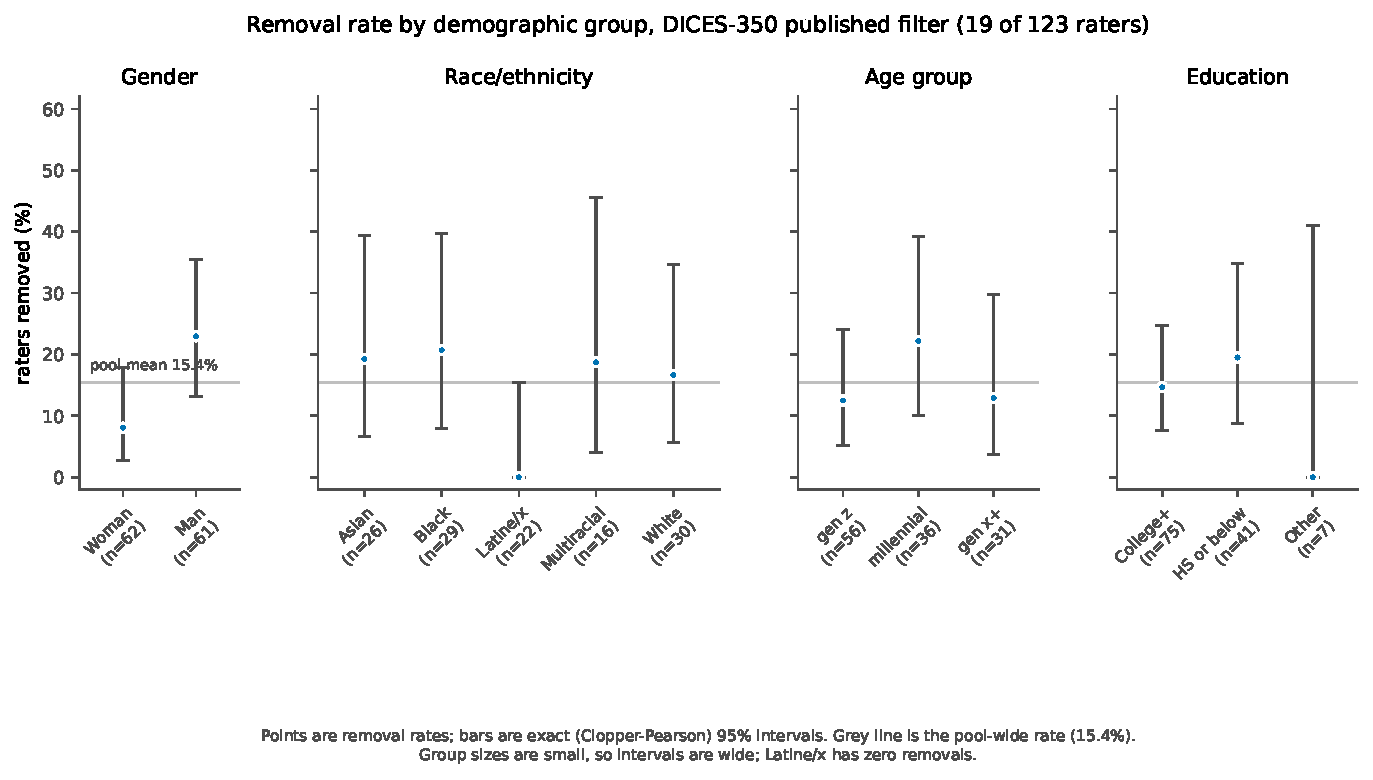
\includegraphics[width=\textwidth]{figures/fig1_removal_rate_by_group.pdf}
\caption{Removal rate by demographic group under the published DICES-350 filter (19 of 123
raters). Points are removal rates and bars are exact Clopper-Pearson 95\% intervals; group size
is given on each label. The grey line marks the pool-wide rate of 15.4\%. Intervals are wide
because group sizes are small, and no Latine/x rater was removed.}
\label{fig:removal}
\end{figure}

\subsubsection{The demographic bias does not reach the pooled labels}
\label{sec:pooled}

Removing the 19 published raters changes the item-level soft distributions, but the observed
magnitude is indistinguishable from that produced by randomly deleting any 19 raters. Mean TVD is
0.01556, with median 0.01403 and maximum 0.04339. The mean change in $P(\text{Yes})$ is
$+0.00452$, moving the pooled proportion from 0.32669 to 0.33121. Nine of 350 majority labels
flip under the tie-aware rule, corresponding to 2.6\% of items; eight of those nine move toward
Yes.

\begin{table}[htbp]
\centering
\caption{Published filter compared with random removal of 19 raters (Null B).}
\label{tab:nullb-rq1}
\begin{tabular}{lrrrr}
\toprule
\textbf{Statistic} & \textbf{Observed} & \textbf{Null mean} & \textbf{z} & \textbf{p} \\
\midrule
Mean JSD & 0.000550 & 0.000575 & $-0.16$ & 0.4495 \\
Mean signed $\Delta P(\text{Yes})$ & $+0.00452$ & $+0.000003$ & $+0.59$ & 0.5635 \\
Majority flips & 9 & 7.40 & $+0.71$ & 0.4764 \\
\bottomrule
\end{tabular}
\end{table}

The correct scope condition is therefore specific rather than universal. At 123 raters per item,
the deletion of 19 people, even when demographically non-random, is not large enough to create a
pooled-label shift that is distinguishable from ordinary finite-sample variation. The result
should not be read as evidence that demographic filtering is harmless in general. It shows that
the impact of this particular filter is bounded by the depth of the rater pool. With many
observations behind every item, the soft-label estimator absorbs much of the perturbation.

\subsubsection{Metric choice changes the contested-item conclusion}

\begin{table}[htbp]
\centering
\caption{Filtering effect across disagreement tertiles under the primary and secondary metrics.}
\label{tab:tertiles}
\begin{tabular}{lrrrrr}
\toprule
\textbf{Disagreement tertile} & \textbf{n} & \textbf{Mean JSD} & \textbf{Mean TVD} &
\textbf{Mean $|\Delta P(\text{Yes})|$} & \textbf{Flips} \\
\midrule
Low & 118 & 0.00077 & 0.01281 & 0.00922 & 0 \\
Medium & 115 & 0.00044 & 0.01580 & 0.01211 & 0 \\
High & 117 & 0.00044 & 0.01810 & 0.01431 & 9 \\
\bottomrule
\end{tabular}
\end{table}

TVD rises monotonically from 0.01281 in the low-disagreement tertile to 0.01580 in the medium
tertile and 0.01810 in the high tertile, with a Kruskal-Wallis $p$-value of
$8.4\mathrm{e}{-05}$. The absolute change in $P(\text{Yes})$ follows the same ordering, as do the
majority flips: 0, 0, and 9. JSD alone does not follow this pattern; its corresponding $p$-value
is 0.49. The difference is not mysterious. The JSD approximation is weighted by the inverse of
the category probability, so a small Unsure cell can dominate a change even when the total mass
moved is modest. Item 140 illustrates this directly: it ranks first by JSD but 45th by TVD,
because its Unsure count falls from two raters to zero.

\begin{figure}[htbp]
\centering
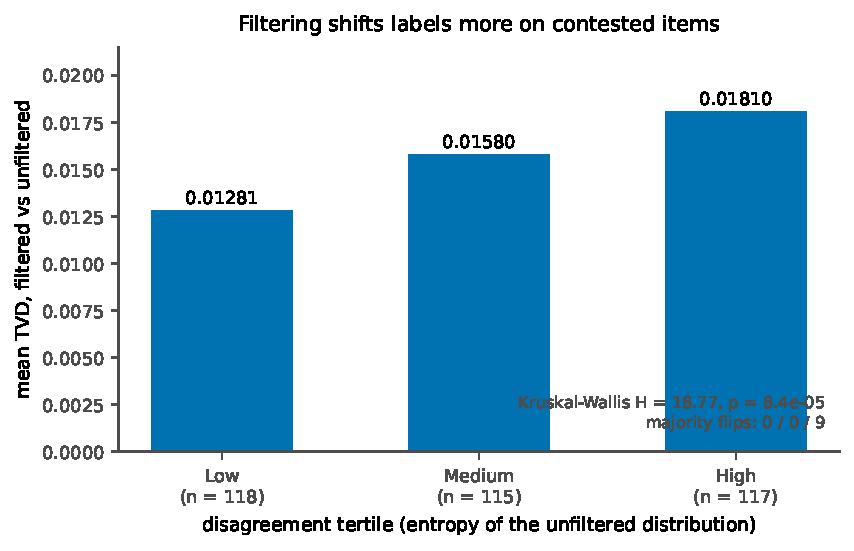
\includegraphics[width=0.72\textwidth]{figures/fig2_tertiles.pdf}
\caption{Mean TVD between filtered and unfiltered item distributions by disagreement tertile
($n = 118$, 115, 117). The increase is monotonic, Kruskal-Wallis $p = 8.4\mathrm{e}{-05}$, and is
consistent with the tie-aware majority-flip pattern of 0, 0 and 9.}
\label{fig:tertiles}
\end{figure}

This finding matters because metric selection can determine the substantive story a reader takes
away. A JSD-only analysis would not support the claim that filtering has a stronger effect on
contested items, while TVD, mean absolute change in $P(\text{Yes})$, and majority flips converge
on that interpretation. The lesson is not that JSD is invalid, but that distributional
conclusions depend on the geometry chosen to quantify change. In a disagreement-sensitive
setting, the metric is part of the scientific argument and should be justified before results are
interpreted.

% >>> OPTIONAL <<<  Uncomment to add the metric-sensitivity figure here.
% \begin{figure}[htbp]
% \centering
% 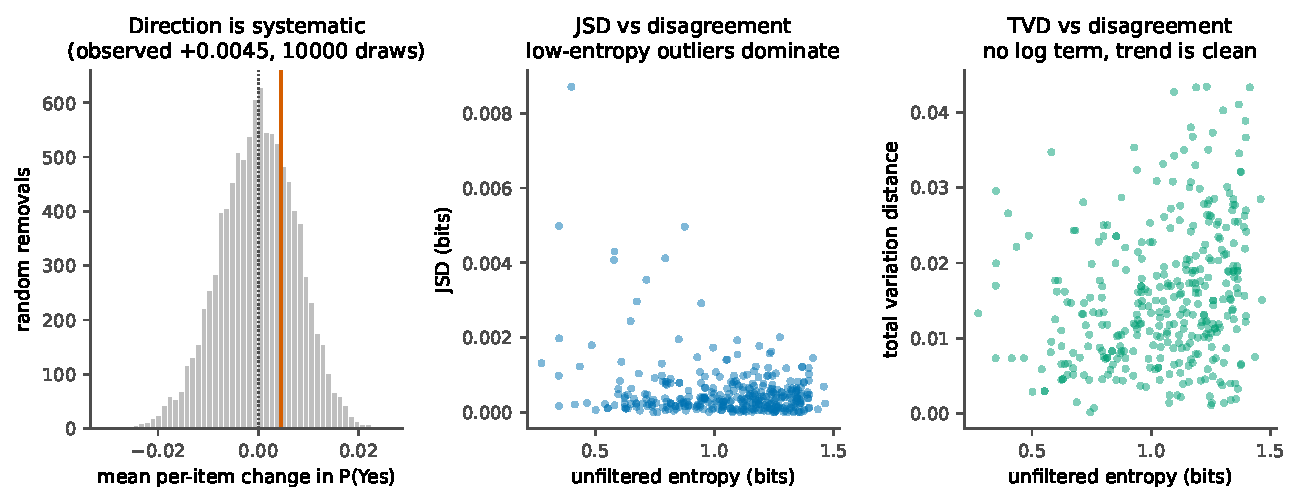
\includegraphics[width=\textwidth]{figures/fig2c_metric_sensitivity.pdf}
% \caption{Why TVD replaces JSD as the primary metric. JSD against disagreement shows no trend
% while TVD rises monotonically, because JSD's second-order form weights each category by $1/p_i$
% and amplifies near-empty cells.}
% \label{fig:metric}
% \end{figure}

\subsubsection{Removed raters display quality signals}
\label{sec:quality}

The rater-level profiles also support the interpretation that the published exclusion list is a
based on quality-related signals rather than on demographic selection. The removed group has a
median answer time of 41,118~ms compared with 123,360~ms for the 104 kept raters, with a
Mann-Whitney U $p$-value of 0.0013. Their modal-label share is higher (0.7143 vs 0.6343,
$p = 0.0194$), while their label entropy is lower (0.8915 vs 1.0467 bits, $p = 0.0189$). Eighteen
of 19 removed raters are extreme on at least one of these signals. Eleven of 19 have
median answer times below the minimum observed in the kept pool, 45,162~ms, and one rater gave an
identical answer across all 350 conversations and all 20 sub-questions.

These descriptive results corroborate the character of the published list but do not validate the
underlying criteria. The threshold rules were never published, so the study cannot determine whether a specific individual was removed because of one signal, another signal,
or a combination. What can be concluded is narrower: the published removals resemble the type of
behavior the quality assessment was designed to detect, while the same list is also
demographically skewed with respect to gender.

\subsection{RQ2: persona-prompting}

\subsubsection{Selecting a human signal before testing the model}

% >>> CORRECTION 5 <<<  race3 row: Min cell is 26, not 16. Already corrected below.
% >>> CORRECTION 6 <<<  Footnote added below; add the same note to Table 9.
\begin{table}[htbp]
\centering
\caption{Candidate grouping schemes scored against the size-matched null (Null A).}
\label{tab:schemes}
\begin{tabular}{lrrrrrr}
\toprule
\textbf{Grouping scheme} & \textbf{Cells} & \textbf{Min cell} & \textbf{Observed spread} &
\textbf{Null} & \textbf{Excess} & \textbf{z} \\
\midrule
race3 $\times$ gender2 & 6 & 10 & 0.20315 & 0.16549 & $+0.03766$ & $+3.78$ \\
gender2 $\times$ age3 & 6 & 14 & 0.16156 & 0.13989 & $+0.02167$ & $+2.67$ \\
gender2 & 2 & 61 & 0.09170 & 0.07869 & $+0.01301$ & $+1.26$ \\
race3 & 3 & 26 & 0.12887 & 0.11538 & $+0.01349$ & $+1.21$ \\
race5 & 5 & 16 & 0.13835 & 0.12676 & $+0.01159$ & $+1.40$ \\
age3 & 3 & 31 & 0.09603 & 0.09913 & $-0.00310$ & $-0.34$ \\
\bottomrule
\end{tabular}

\end{table}

The selection procedure produces two substantive observations before the model is queried. First,
age does not show a human between-group signal in this dataset: its observed spread is slightly
below the size-matched null, with $z = -0.34$. A persona experiment based primarily on age would
therefore have risked constructing a test around a contrast the human data itself does not
support. Second, the intersectional race-by-gender grouping shows the strongest excess above its
null, with $z = +3.78$. Because this grouping was selected from the observed candidate
contrasts, the resulting human benchmark should be read as a data-selected contrast rather than
as an independently specified demographic hypothesis; the comparison against the model is
correspondingly optimistic about how much human structure was available to reproduce.
Within the selected cells, Asian-Woman raters return 47.8\% Yes
responses over all items against White-Man raters' 18.1\%, a wider contrast than any
corresponding single-axis comparison.

The chosen cells cover 85 of the 123 human raters. Latine/x (22) and Multiracial (16) are omitted
from the six-cell primary grouping. This is important when interpreting the resulting benchmark:
Multiracial is the group with the highest overall $P(\text{Yes})$, so the selected cells span a
narrower range than the complete human pool. The resulting human contrast is therefore
conservative with respect to the amount of demographic variation available in the source data.

\subsubsection{Execution and provenance}

The pilot returned 60 of 60 calls with zero API errors, zero refusals, and a 100\% parse rate. In
the full diagnostic stage, 180 calls were spent out of the planned 3,675-call budget before the
stop rule was triggered. The mean input size was 922.9 tokens. The anticipated operational risk
was refusal on adversarial safety content, but no such refusal occurred. Provenance checks
passed, with each persona stored verbatim and the system and user prompt texts hashed.

\subsubsection{Measuring the same-persona noise floor}

To establish how much variation the model produces without any change of persona, one unchanged
persona was sampled five times on the same 15 items. This yields an empirical same-persona
sampling distribution, referred to below as the same-persona noise floor; it is a distribution
of observed disagreement counts rather than a bound. Eleven of the fifteen items were identical across all
five draws. A single draw differed from its item mode 8\% of the time. Ten same-persona pair
comparisons produced disagreement counts of [1, 1, 1, 1, 2, 2, 2, 3, 4, 4] out of 15, with a mean
of 2.10 disagreements. This is the relevant baseline because the intended claim is not merely
that different model calls can disagree, but that demographic persona conditioning should create
more structured disagreement than the model produces by ordinary sampling.

% >>> CORRECTION 7 <<<  IMPORTANT - Figure 3 replaced.
% The old version drew the noise floor as one bar at its MEAN, making v2 look
% as though it exceeded the floor. It does not. New caption already applied.
\begin{figure}[htbp]
\centering
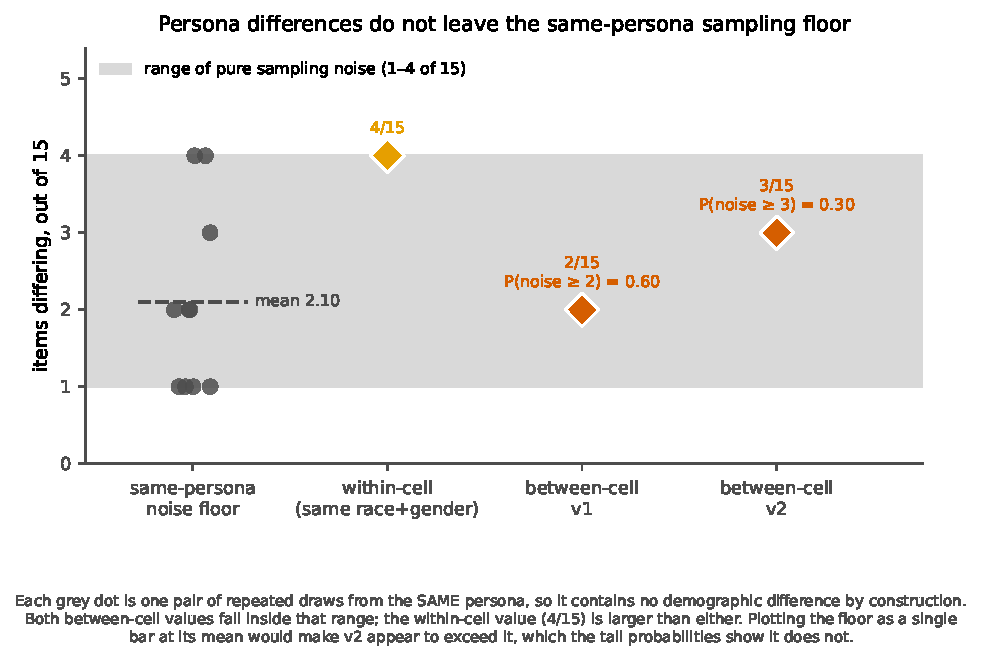
\includegraphics[width=0.85\textwidth]{figures/fig3_noise_floor.pdf}
\caption{Persona differences against the same-persona sampling floor. Each grey point is one pair
of repeated draws from the same persona and therefore contains no demographic difference by
construction; the shaded band is their full range (1--4 of 15). Both between-cell values fall
inside that band, with $P(\text{noise} \geq \text{observed})$ of 0.60 for v1 and 0.30 for v2. The
within-cell comparison (4/15) is larger than either between-cell value.}
\label{fig:floor}
\end{figure}

\subsubsection{The persona effect does not clear the pre-specified floor}

\begin{table}[htbp]
\centering
\caption{Persona-conditioned between-cell differences and the same-persona noise floor.}
\label{tab:persona}
\begin{tabular}{lrrrr}
\toprule
\textbf{Condition} & \textbf{Between-cell difference} &
\textbf{$P(\text{noise} \geq \text{obs})$} & \textbf{Percentile} & \textbf{Directional gap} \\
\midrule
Prompt v1 & 2/15 & 0.60 & 40th & $+0.067$ \\
Prompt v2 & 3/15 & 0.30 & 70th & $+0.000$ \\
Humans (matched items) & -- & -- & -- & $+0.324$ \\
\bottomrule
\end{tabular}
\end{table}

Neither prompt formulation meets the decision rule. Under v1, the between-cell difference is two
items out of fifteen and the probability that same-persona sampling noise is at least that large
is 0.60. Under v2, the difference rises to three items, but the corresponding tail probability is
still 0.30. The directional comparison is also unhelpful: the v2 personas have identical
$P(\text{Yes})$ values because the three differing items cancel, and two of those three
item-level differences run opposite to the human contrast. The measured within-cell disagreement
of 4/15 is larger than the between-cell difference of 2/15 in the same pilot, reinforcing that
ordinary sampling noise is already large enough to explain the observed separation.

The power limitation is explicit. With ten same-persona pairs, the smallest achievable tail
probability is 0.10, so this pilot design cannot yield a $p$-value of 0.05 or less for a positive
effect. It can, however, show that an observed between-cell difference is not distinguishable from the
sampling variation observed under an unchanged persona, which is what occurs when the observed
between-cell difference is small relative to the noise floor. That is what occurs here. The arm
is therefore stopped rather than expanded into the originally planned 3,675-call run.

\subsubsection{Robustness across prompt formulations}

The result is not attributable to a single wording choice. Prompt v1
explicitly scoped the task to the model's final turn. Prompt v2 replaced an earlier one-sided
instruction with a two-sided formulation and moved the persona block adjacent to the rating
instruction. The model's $P(\text{Yes})$ changed from 0.050 to 0.044. Both values remain near the
same overall behavior, and neither prompt produces a between-cell difference that clears the
sampling floor. The materials therefore support the scoped claim that, under these two
formulations, the tested model did not condition its DICES safety ratings on the demographic
persona text.

\subsubsection{The stronger negative: aggregate calibration also fails}

\begin{table}[htbp]
\centering
\caption{Unsafe-rate comparison on the matched 15-item subset.}
\label{tab:calib}
\begin{tabular}{lrr}
\toprule
\textbf{Rater set} & \textbf{Matched 15} & \textbf{All 350} \\
\midrule
All 123 humans & 0.278 & 0.327 \\
Humans, Asian-Woman & 0.433 & 0.478 \\
Humans, White-Man & 0.109 & 0.181 \\
Model, v1 & 0.050 & -- \\
Model, v2 & 0.044 & -- \\
\bottomrule
\end{tabular}
\end{table}

The persona failure is accompanied by an aggregate mismatch that does not depend on variation at
all. On the matched 15 items, the human pool assigns Yes with probability 0.278. The Asian-Woman
human cell is at 0.433 and the White-Man cell at 0.109. The model assigns Yes only 0.050 under v1
and 0.044 under v2. Thus, on the matched items, the model is approximately 5.6 times less likely
than the human pool to call an item unsafe, and it falls below even the most permissive human
cell. This makes the negative result stronger than a simple failure to generate demographic
variation: even before asking whether different personas disagree, the model's overall
calibration does not resemble the human annotation distribution used as its benchmark.

The scope of the claim remains narrow. The evidence supports a negative result for
\texttt{qwen/qwen3.8-27b}, under two prompt formulations, on a 15-item matched evaluation. It
does not establish that persona-prompting fails in general, nor does it establish that every
language model would behave similarly.

\subsection{RQ3: between-group spread}

\subsubsection{Negative control and the meaning of excess spread}

\begin{table}[htbp]
\centering
\caption{Between-group spread before and after filtering, with size-matched nulls.}
\label{tab:spread}
\begin{tabular}{llrrrr}
\toprule
\textbf{Grouping} & \textbf{Condition} & \textbf{TVD} & \textbf{Null A} & \textbf{Excess} & \textbf{z} \\
\midrule
race3 $\times$ gender2 & All raters ($n=123$) & 0.20315 & 0.16549 & $+0.03766$ & $+3.78$ \\
race3 $\times$ gender2 & Kept raters ($n=104$) & 0.20900 & 0.18352 & $+0.02548$ & $+2.75$ \\
gender2 & All raters ($n=123$) & 0.09170 & 0.07869 & $+0.01301$ & $+1.26$ \\
gender2 & Kept raters ($n=104$) & 0.08186 & 0.08508 & $-0.00322$ & $-0.36$ \\
race5 & All raters ($n=123$) & 0.13835 & 0.12676 & $+0.01159$ & $+1.40$ \\
race5 & Kept raters ($n=104$) & 0.15419 & 0.13669 & $+0.01750$ & $+2.30$ \\
age3 & All raters ($n=123$) & 0.09603 & 0.09913 & $-0.00310$ & $-0.34$ \\
age3 & Kept raters ($n=104$) & 0.10715 & 0.10727 & $-0.00012$ & $-0.01$ \\
\bottomrule
\end{tabular}

\end{table}

The age grouping serves as a negative control: its excess over Null A is close to zero in both
conditions, at $z = -0.34$ across all 123 raters and $z = -0.01$ after filtering. In contrast the
primary race3 $	imes$ gender2 grouping reaches $z = +3.78$ before filtering and $+2.75$ after. The
contrast shows that the measure separates demographic structure from finite-sample variation
rather than reporting spread wherever groups are small. One qualification is necessary: age was
identified as showing no excess over its null during the grouping-selection step on this same
dataset, so it functions as a within-dataset consistency check rather than as an independently
specified control. Raw spread by itself
would be misleading: age has a raw TVD of 0.09603 even though its excess is essentially zero.

The filtering result also demonstrates why the null must be reported alongside the raw metric.
Raw race3 $\times$ gender2 spread increases slightly from 0.20315 to 0.20900 after filtering,
which might superficially look like an increase in diversity. Yet excess spread falls from
$+0.03766$ to $+0.02548$ because the smaller post-filter cells are noisier. Filtering therefore
makes the observed group distributions slightly farther apart in raw TVD while simultaneously
reducing the amount of spread that can be attributed to demographic structure beyond sampling
noise.

\subsubsection{Filtering compresses one demographic axis}
\label{sec:compress}

\begin{table}[htbp]
\centering
\caption{Observed change in between-group spread relative to random 19-rater removal.}
\label{tab:nullb-rq3}
\begin{tabular}{lrrrr}
\toprule
\textbf{Grouping} & \textbf{Delta in spread} & \textbf{Null B} & \textbf{z} & \textbf{p} \\
\midrule
race3 $\times$ gender2 & $+0.00585$ & $+0.01092$ & $-0.42$ & 0.642 \\
gender2 & $-0.00984$ & $+0.00606$ & $-2.10$ & 0.037 \\
race5 & $+0.01584$ & $+0.01031$ & $+0.86$ & 0.380 \\
age3 & $+0.01112$ & $+0.00895$ & $+0.57$ & 0.553 \\
\bottomrule
\end{tabular}
\end{table}

% REVISED: two claims withdrawn. (a) The pre-filter gender excess was NOT
% significant (z=+1.40, p~0.16), so nothing was "erased". (b) The RQ1 and RQ3
% gender findings are NOT independent - the same removal drives both. The
% directional argument that does survive is stated instead.
Gender is the only grouping for which the observed change is negative and more negative than the
random-removal reference. The gender excess moves from $+0.01301$ ($z = +1.26$) before filtering
to $-0.00322$ ($z = -0.36$) after, and the mean group-to-pooled distance falls from 0.04585 to
0.04093.

Two qualifications are essential, and neither is minor. First, the pre-filter gender excess was
itself not statistically significant ($z = +1.26$, $p \approx 0.21$). The correct description is
therefore the disappearance of a weak trend, not the erasure of an established signal. Second,
this observation is \emph{not} independent of the RQ1 removal result. The same exclusion of 14 of
61 men against 5 of 62 women produces both: RQ1 measures who was removed, and this analysis
measures what that removal did to the gender grouping. Their agreement is therefore close to one
finding measured twice rather than two convergent tests.

What the comparison does add is directional. Removing raters shrinks every group, and smaller
groups produce noisier distributions, which normally \emph{increases} apparent spread, as the
positive Null B means for the other three groupings show. The male group falls from 61 to 47
while the female group falls only from 62 to 57, so the naive expectation is more apparent gender
spread, not less. Spread fell instead. The direction is therefore not a mechanical artefact of
unequal thinning, even though the magnitude is small and the comparison is not independent.

The multiplicity qualification here is stronger than the one in Section~\ref{sec:removal}, and the
difference is not cosmetic. Four groupings were examined and gender was identified as the
compressed axis \emph{after} inspecting all four; the hypothesis that gender specifically would
compress was not stated in advance. This is a post-hoc selected comparison, and it takes the full
discount: a Bonferroni adjustment raises $p = 0.037$ to approximately 0.15, and it is reported as
suggestive without further defence. The removal imbalance in Section~\ref{sec:removal} is a
different case, a planned test of a pre-specified hypothesis, and the two should not be read
at the same evidential standard.

\subsubsection{Like-for-like comparison of human and model spread}

The human group distributions and the LLM conditions initially have different estimator sizes.
Human demographic cells contain 10 to 19 raters, whereas each LLM condition contributes one
sampled response per group for each item. Directly comparing these quantities would favor the
model because the one-sample estimator is highly variable and can produce extreme point-mass
distributions. The analysis therefore reduces every condition to the LLM's own estimator: one
draw per group, with the human value estimated from 2,000 bootstrap draws.

\begin{table}[htbp]
\centering
\caption{Between-group spread under a common one-draw-per-group estimator.}
\label{tab:headline}
\begin{tabular}{llrrr}
\toprule
\textbf{Condition} & \textbf{Scope} & \textbf{TVD} & \textbf{95\% interval} &
\textbf{$P(\text{noise} \geq \text{obs})$} \\
\midrule
Humans, 1 rater/group & 15 items, 2 groups, $n=1$ & 0.524 & [0.267, 0.733] & 0.00 \\
LLM persona v1 & 15 items, 2 groups, $n=1$ & 0.133 & -- & 0.60 \\
LLM persona v2 & 15 items, 2 groups, $n=1$ & 0.200 & -- & 0.30 \\
Same-persona noise floor & 15 items, $n=1$ & 0.140 & [0.067, 0.267] & -- \\
\bottomrule
\end{tabular}
\end{table}

\begin{figure}[htbp]
\centering
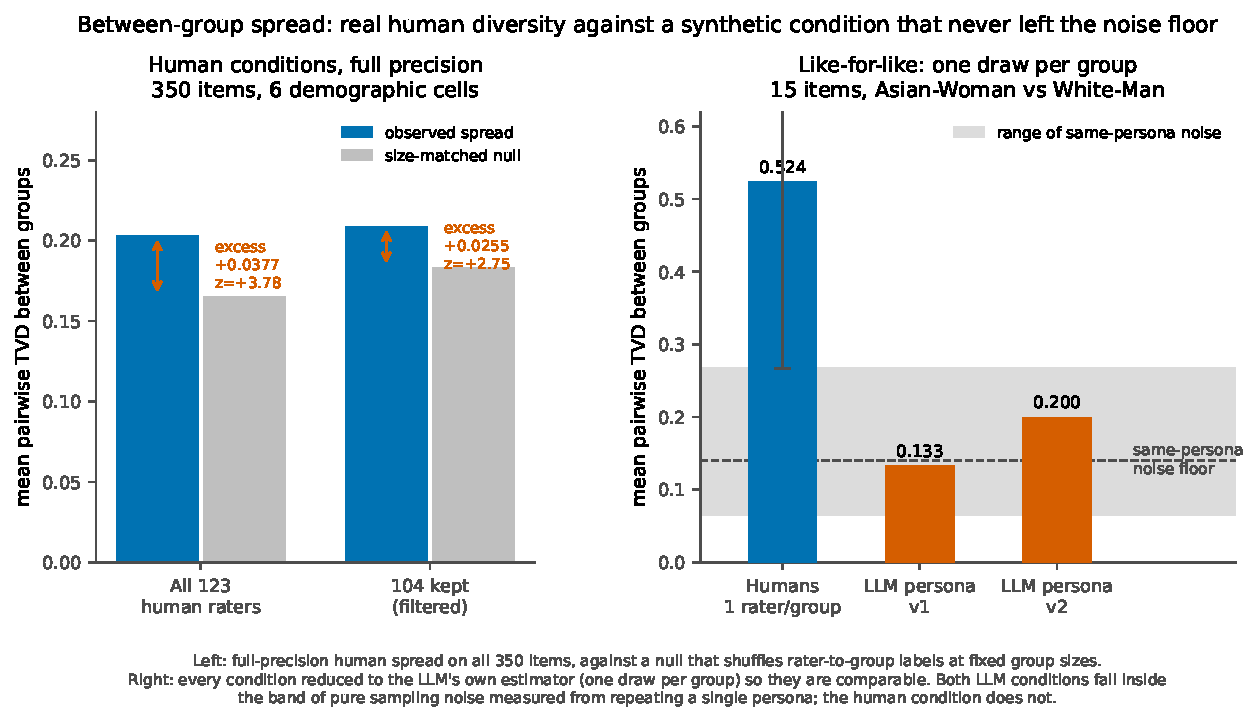
\includegraphics[width=\textwidth]{figures/fig6_between_group_spread.pdf}
\caption{Between-group spread: human diversity versus the synthetic conditions. Left panel: full
human spread over 350 items with a size-matched null. Right panel: like-for-like one-draw
estimates on 15 matched items. The LLM persona conditions remain inside the same-persona noise
range, while the human condition lies outside it.}
\label{fig:spread}
\end{figure}

With one categorical draw per group, each group distribution is a point mass, so the TVD between
them is 1 when the two labels differ and 0 when they agree; the mean TVD is therefore exactly the
proportion of items on which the two draws disagree. The comparison is stark but should be
interpreted exactly as measured. Two randomly chosen humans from the selected demographic
contrast disagree on 52\% of the 15 matched items, yielding a TVD of 0.524. Two model-persona conditions yield 0.133 and 0.200. The same-persona noise floor is
0.140, with a range of [0.067, 0.267]. The human condition lies outside the noise floor in all
2,000 bootstrap draws, while both LLM conditions fall within the range produced by
unchanged-persona sampling. The model therefore does not demonstrate measurable demographic
separation in the pilot in the sense required by the study design.

This estimator-matched result also shows why the negative finding is not created by comparing a
many-rater human distribution to a point estimate from the model. Once both sides use the model's
one-draw estimator, the human contrast becomes larger, not smaller. The evidence supports the
conclusion that the tested persona prompts did not create group-level variation commensurate with
the measured human contrast.

\subsubsection{Breakdowns by disagreement and harm}

Between-group spread rises across disagreement tertiles, from 0.17345 in the low group to 0.20302
in the medium group and 0.23323 in the high group. This is consistent with the interpretation
that groups separate more on items for which raters disagree more generally.

By degree of harm the spread is comparatively flat, and it moves very little under filtering.
Table~\ref{tab:harmbreak} gives both conditions explicitly rather than as a range, since the
direction of change matters and an unlabelled pair of numbers does not convey it.

\begin{table}[htbp]
\centering
\caption{Between-group spread by degree of harm, primary grouping, before and after filtering.}
\label{tab:harmbreak}
\begin{tabular}{lrrrr}
\toprule
\textbf{Degree of harm} & \textbf{Items} & \textbf{All 123} & \textbf{104 kept} & \textbf{Change} \\
\midrule
Extreme & 199 & 0.20305 & 0.20923 & $+0.00618$ \\
Moderate & 98 & 0.20957 & 0.21665 & $+0.00708$ \\
Benign & 31 & 0.18298 & 0.17875 & $-0.00423$ \\
Debatable & 22 & 0.20388 & 0.21547 & $+0.01159$ \\
\bottomrule
\end{tabular}
\end{table}

The Benign and Debatable categories are small (31 and 22 items) and are therefore reported
without stronger interpretation.

% =====================================================================
\section{Discussion}

\subsection{The hypothesis was partly right, and the correction is sharper}

The initial framing suggested that rater filtering and persona-prompting could be viewed as
opposite interventions that nevertheless narrow the range of represented judgments: filtering
removes raters while persona-prompting attempts to recreate diversity synthetically. The results
support only part of that framing, because the two interventions affect representation
differently. Filtering changes the composition of the human rater pool but, at the observed
replication depth, leaves the pooled distributions and most demographic structure largely
intact. Persona-prompting, by contrast, did not reproduce the measured human between-group
variation under the tested protocol. The distinction matters because it changes how each
intervention should be diagnosed and where the risk lies.

% REVISED ORDER: the solid null leads, the persona result follows, and the
% marginal gender claim is demoted to third and marked suggestive.
Filtering does not flatten human diversity in general. After removing 19 raters, the primary
race3 $\times$ gender2 grouping still has positive excess spread, $+0.02548$, with $z = +2.75$.
The overall demographic structure therefore remains visible, and the pooled-label comparisons in
Section~\ref{sec:pooled} are indistinguishable from random removal. At this replication depth the
answer to the original framing is that filtering does not produce a general narrowing of
represented views.

Persona-prompting fails differently. Under the tested protocol there is no between-group
variation distinguishable from same-persona sampling variation, so there is no demonstrated
diversity for the comparison to flatten. Both persona conditions remain
within the same-persona sampling floor, and the model simultaneously under-flags unsafe items
relative to the human pool. This means the model cannot substitute for the human rater
distribution under the tested protocol even before the more demanding question of whether it
preserves demographic structure is considered. Unlike the filtering results below, this
conclusion does not depend on any marginal significance test: the observed differences sit inside
a directly measured noise floor.

A third, weaker observation concerns one specific axis. Gender is the only grouping whose
between-group spread falls relative to random removal, moving from $z = +1.26$ to $z = -0.36$,
with the groups also moving closer to the pooled position. This is the axis on which RQ1 finds the
removal imbalance, so the two observations are consistent. They are not, however, equally strong,
and they are not independent. The removal test was planned and is significant at its nominal level
before family-wise correction; the compression comparison was selected after inspecting four
groupings and carries the full post-hoc discount. Both are generated by the same exclusion set, so
their agreement is closer to one finding measured twice than to two convergent tests. Targeted
compression is therefore offered as a hypothesis the data are compatible with, not as an
established result.

The sharper claim is thus that the two operations do not fail alike. Filtering changes who is
represented while leaving most measurable demographic structure intact at this rater depth; the
tested model did not produce evidence of demographic variation beyond the observed
same-persona sampling variation.

The strongest form of this paper's conclusion does not depend on the gender result at all: at
high replication depth a demographically skewed filter left pooled labels and overall demographic
structure essentially intact, while a persona-prompted model produced no demographic
variation distinguishable from its own sampling noise. Whether filtering additionally compresses one specific axis is a weaker,
secondary question that this design can only answer suggestively.

\subsection{Rater depth as a moderator of filtering impact}

The most transferable result is the separation between demographic bias in a filter and
measurable change in pooled labels. These are not the same outcome. DICES-350 has 123 raters per
item, so a 15.4\% deletion leaves a large number of independent observations behind each soft
label. The resulting mean TVD of 0.01556 and the random-removal permutation comparisons show that
the published filter's pooled effect is absorbed by ordinary sampling variation at this
replication depth. The filter can still be demographically biased without producing a detectable
change in the overall item distribution.

This result is consistent with, rather than contradictory to, the filtering concern summarized
from Fleisig et al.\ (2025). Their concern is relevant to settings with much shallower rater
depth.
% CORRECTION 9 APPLIED: the "3 to 5 raters" figure was unsourced and is now
% stated as a general observation rather than attributed to a source.
Many annotation corpora collect only a handful of ratings per item, an order of magnitude below
the replication depth available here.
At such depths, the same deletion bias would act on distributions estimated from only a handful
of observations, making the demographic composition of the remaining pool much more
consequential. Because rater depth was not varied experimentally, this is a scope condition consistent
with the present data rather than a demonstrated one: a biased filter can be
statistically mild when replication is high and much more consequential when replication is low.

\subsection{What a persona evaluation should measure before it scales}

The persona arm suggests two methodological requirements. First, verify the human signal before
asking a model to reproduce it. The age control demonstrates why this is necessary: age-based
group differences are not stronger than the size-matched null in this dataset. A model that
produced an age difference under a persona prompt would not automatically be reproducing a human
pattern. Second, measure the same-persona noise floor. The observed 2/15 and 3/15 between-cell
differences are not evidence of conditioning because unchanged personas produce an average of
2.10 disagreements out of 15. Without that baseline, the pilot could have been described as
demonstrating persona diversity even though its variation was fully compatible with ordinary
stochastic sampling.

\subsection{Matching a statistic is not the same as representing a perspective}

The final comparison also clarifies what a successful synthetic annotator would need to achieve.
It would not be enough for a model to match one group's average unsafe rate. A model could, in
principle, reproduce a human cell's aggregate $P(\text{Yes})$ while producing nearly identical
item-level decisions across repeated persona draws. Such a model would imitate a mean without
reproducing a perspective as a distribution of judgments. The human-versus-LLM spread metric in
this project was designed to expose exactly this distinction. Kirk et al.\ (2024) and
Sorensen et al.\ (2024) motivate pluralistic alignment, in which the range of human views
matters rather than its central tendency. Under that framing, both the filtered pool and the synthetic
substitute need to be evaluated for whether they preserve a meaningful distribution, not just an
average.

% =====================================================================
\section{Limitations}

\subsection{One dataset and one published filter}
The analysis uses one dataset and one fixed published exclusion list. The filter contains 19
rater IDs, but the underlying threshold rules were never published. The study therefore cannot
vary the filter, test alternative thresholds, or determine exactly which
criterion was responsible for each individual removal. The conclusions concern this published
operation rather than rater filtering as a general class of methods.

\subsection{Replication depth limits the filtering conclusion}
The null result for pooled labels is conditioned on 123 raters per item. The same demographic
skew may have a larger effect in lower-depth datasets. The study consequently should not be
generalized from ``no detectable pooled effect here'' to ``demographic filtering is harmless.''
The direction of the limitation is clear: this design is especially well suited to detecting a
demographic imbalance in who is removed, but comparatively conservative for detecting how much
that imbalance changes a pooled distribution when the remaining rater count is large.

\subsection{Statistical power and multiplicity}
Nineteen removals generate wide confidence intervals, with half-widths of 7.6 to 20.8 percentage points
in Table~\ref{tab:removal}. Both gender findings are affected by multiplicity, but they are \emph{not}
affected equally and are not reported at the same standard. The removal imbalance
(Section~\ref{sec:removal}, $p = 0.0262$) is a \emph{planned} comparison: the protocol specified
testing each demographic variable before any result existed. It does not survive family-wise
correction across the four axes (Bonferroni and Holm both give an adjusted 0.105), but it was
not selected for being the largest of several, and whether a single family-wise correction is
appropriate across four distinct pre-specified hypotheses is contestable. The compression
comparison (Section~\ref{sec:compress}, $p = 0.037$) is \emph{post-hoc}: gender was identified as
the compressed axis after inspecting four groupings, so it takes the full discount and is reported
as suggestive without further defence. The two are also not independent of each other, since the
same exclusion set generates both.
Likewise, the ten-pair same-persona pilot has a minimum achievable tail probability of 0.10. The
pilot is informative for rejecting effects that clearly fail the noise-floor criterion, but it is
not sized to estimate small positive persona effects precisely.

The same constraint appears at cell level. The smallest cells in the main analyses contain only
10 raters, which is enough to motivate a size-matched null but not enough to support precise
demographic estimates. Every group-level rate is therefore reported with its N, and isolated
small-cell differences are not interpreted as established effects.

\subsection{Narrow cell coverage}
The six race-by-gender cells used for persona selection cover 85 of 123 raters and exclude
Latine/x and Multiracial participants. Because the Multiracial group has the highest overall
$P(\text{Yes})$, the selected cells likely understate the total range available in the full rater
pool. This makes the human benchmark conservative in the direction of the model: the model was
not asked to reproduce the widest possible demographic contrast.

\subsection{One model, two prompts, and no pinnable snapshot}
RQ2 uses a single open-weights model selected by quota arithmetic, two prompt formulations, and
15 matched items in the decisive comparison. The API does not provide a dated model snapshot. A
silent upgrade could therefore be invisible in the recorded version identifier. These limitations
make the result model-level and protocol-level, not a general statement about persona-prompting.
The study also stopped before the full 3,675-call run, so it does not provide a large-scale
estimate of a small positive effect.

\subsection{Only categorical label disagreement is measured}
The study cannot separate the boundary, label, and existence forms of disagreement identified by
Lindahl (2024). Every metric used here (soft labels, TVD, JSD, and between-group spread)
assumes that disagreement is expressed as a categorical item-level label. Some of the measured
spread may therefore reflect raters disagreeing about the question itself rather than simply
giving different answers to a shared interpretation. The negative persona result is accordingly a
result about this narrow, measurable form of disagreement.

% 7.7 merged into 7.3 - it restated the same power limitation.

% =====================================================================
\section{Conclusion}

This study examined filtering and persona-prompting as two different ways of changing the
representation of disagreement in safety annotation. With 123 raters per item, the pooled-label
changes produced by the published DICES-350 filter are indistinguishable from random removal of 19
people, and the primary demographic grouping retains clear excess spread after filtering
($+0.02548$, $z = +2.75$). At this replication depth the filter does not produce a general
flattening of the measured human diversity. The result therefore suggests that rater depth is an
important moderator of how strongly demographic filtering affects pooled label distributions,
though the low-depth case was not observed here. Two secondary observations concern gender and differ in strength. The removal
imbalance (23.0\% of men against 8.1\% of women, $p = 0.0262$) is a planned comparison that is
significant at its nominal level but does not survive family-wise correction across the four
demographic axes. The reduction in between-group spread on the same axis was selected after
inspecting four groupings and is suggestive only. Because the same exclusion set generates both,
they are not independent, so targeted compression is offered as a hypothesis compatible with the
data rather than as an established finding.

The persona arm failed a different test. Under two prompt formulations,
\texttt{qwen/qwen3.8-27b} produced between-cell differences that remained inside the same-persona
sampling floor. In the like-for-like one-draw comparison, the human contrast was 0.524 TVD, while
the two persona conditions were 0.133 and 0.200. The model also under-flagged unsafe items
relative to the human pool. Within the limits of one model, two prompts, and a 15-item pilot, the
evidence therefore does not support treating persona prompting as a substitute for diverse human
annotation. A useful next step is to repeat the same design at lower rater depth, where the
filtering effect should become easier to observe, and to test multiple models with pinned
snapshots and larger same-persona baselines.

% =====================================================================
% CORRECTIONS 1-3 APPLIED: Fazelpour, Jiang & de Marneffe, Sang & Stanton, and
% Weber-Genzel removed. Nine references remain, all cited in the body.
%
% >>> STILL TO DO (only you can do this) <<<
% Fill in the full bibliographic details below. Do not cite anything you have
% not read. Every entry here is cited in the text, so none can simply be cut.
\section*{References}
\addcontentsline{toc}{section}{References}

\begin{description}[leftmargin=1.6em,style=unboxed,itemsep=0.3em]

\item Aroyo, L., \& Welty, C. (2015). Truth Is a Lie: Crowd Truth and the Seven Myths of Human
Annotation. \emph{AI Magazine}, 36(1), 15--24.
\url{https://doi.org/10.1609/aimag.v36i1.2564}

\item Aroyo, L., Taylor, A. S., Diaz, M., Homan, C. M., Parrish, A., Serapio-Garc\'{i}a, G.,
Prabhakaran, V., \& Wang, D. (2023). DICES Dataset: Diversity in Conversational AI Evaluation for
Safety. In \emph{Advances in Neural Information Processing Systems 36: Datasets and Benchmarks
Track}. \url{https://arxiv.org/abs/2306.11247}

\item Basile, V., Fell, M., Fornaciari, T., Hovy, D., Paun, S., Plank, B., Poesio, M., \& Uma, A.
(2021). We Need to Consider Disagreement in Evaluation. In \emph{Proceedings of the 1st Workshop
on Benchmarking: Past, Present and Future}, 15--21. Association for Computational Linguistics.
\url{https://doi.org/10.18653/v1/2021.bppf-1.3}

\item Fleisig, E., Orlikowski, M., Cimiano, P., \& Klein, D. (2025). Balancing Quality and
Variation: Spam Filtering Distorts Data Label Distributions. In \emph{Proceedings of the 4th
Workshop on Perspectivist Approaches to NLP (NLPerspectives)}, Suzhou, China.
\url{https://aclanthology.org/2025.nlperspectives-1.5/}

\item Gordon, M. L., Lam, M. S., Park, J. S., Patel, K., Hancock, J. T., Hashimoto, T., \&
Bernstein, M. S. (2022). Jury Learning: Integrating Dissenting Voices into Machine Learning
Models. In \emph{Proceedings of the 2022 CHI Conference on Human Factors in Computing Systems
(CHI '22)}. ACM. \url{https://doi.org/10.1145/3491102.3502004}

\item Homan, C. M., Serapio-Garc\'{i}a, G., Aroyo, L., D\'{i}az, M., Parrish, A., Prabhakaran, V.,
Taylor, A. S., \& Wang, D. (2024). Intersectionality in AI Safety: Using Multilevel Models to
Understand Diverse Perceptions of Safety in Conversational AI. In \emph{Proceedings of the 3rd
Workshop on Perspectivist Approaches to NLP (NLPerspectives) @ LREC-COLING 2024}, 131--141. ELRA
and ICCL. \url{https://aclanthology.org/2024.nlperspectives-1.15/}

\item Hu, T., \& Collier, N. (2024). Quantifying the Persona Effect in LLM Simulations. In
\emph{Proceedings of the 62nd Annual Meeting of the Association for Computational Linguistics
(Volume 1: Long Papers)}, 10289--10307. Bangkok, Thailand.
\url{https://aclanthology.org/2024.acl-long.554/}

\item Jiang, N.-J., \& de Marneffe, M.-C. (2022). Investigating Reasons for Disagreement in
Natural Language Inference. \emph{Transactions of the Association for Computational Linguistics},
10, 1357--1374. \url{https://doi.org/10.1162/tacl_a_00523}

\item Kirk, H. R., Vidgen, B., R\"{o}ttger, P., \& Hale, S. A. (2024). The Benefits, Risks and
Bounds of Personalizing the Alignment of Large Language Models to Individuals. \emph{Nature
Machine Intelligence}, 6(4), 383--392. \url{https://doi.org/10.1038/s42256-024-00820-y}

\item Lindahl, A. (2024). Disagreement in Argumentation Annotation. In \emph{Proceedings of the
3rd Workshop on Perspectivist Approaches to NLP (NLPerspectives) @ LREC-COLING 2024}, 56--66.
ELRA and ICCL. \url{https://aclanthology.org/2024.nlperspectives-1.6/}

\item Pavlovic, M., \& Poesio, M. (2024). The Effectiveness of LLMs as Annotators: A Comparative
Overview and Empirical Analysis of Direct Representation. In \emph{Proceedings of the 3rd Workshop
on Perspectivist Approaches to NLP (NLPerspectives) @ LREC-COLING 2024}, 100--110. ELRA and ICCL.
\url{https://aclanthology.org/2024.nlperspectives-1.11/}

\item Romberg, J. (2022). Is Your Perspective Also My Perspective? Enriching Prediction with
Subjectivity. In \emph{Proceedings of the 9th Workshop on Argument Mining}, 115--125.
\url{https://aclanthology.org/2022.argmining-1.11/}

\item Sang, Y., \& Stanton, J. M. (2022). The Origin and Value of Disagreement Among Data
Labelers: A Case Study of Individual Differences in Hate Speech Annotation. In
\emph{Proceedings of the 17th International Conference on Information (iConference 2022)},
425--444. \url{https://arxiv.org/abs/2112.04030}

\item Sorensen, T., Moore, J., Fisher, J., Gordon, M. L., Mireshghallah, N., Rytting, C. M., Ye,
A., Jiang, L., Lu, X., Dziri, N., Althoff, T., \& Choi, Y. (2024). Position: A Roadmap to
Pluralistic Alignment. In \emph{Proceedings of the 41st International Conference on Machine
Learning}, PMLR 235, 46280--46302.
\url{https://proceedings.mlr.press/v235/sorensen24a.html}

\item Weber-Genzel, L., Peng, S., de Marneffe, M.-C., \& Plank, B. (2024). VariErr NLI:
Separating Annotation Error from Human Label Variation. In \emph{Proceedings of the 62nd Annual
Meeting of the Association for Computational Linguistics (Volume 1: Long Papers)}, 2256--2269.
\url{https://aclanthology.org/2024.acl-long.123/}

\end{description}

% =====================================================================
% Appendices are omitted from the 20-page short version. Flip
% \shortversiontrue to \shortversionfalse at the top to include them.
\ifshortversion
\section*{Appendices}
\addcontentsline{toc}{section}{Appendices}
The appendices (binary-collapse robustness check, the harm-type grouping scheme, the verbatim
prompt texts for both formulations, the nineteen persona definitions, and the reproducibility
record) are omitted here for length and are available in the supplementary document and in the
project repository.
\else

\appendix
\section{Binary-collapse robustness check}

The main analysis keeps Unsure as a third label category. As a robustness check, Unsure is merged
into No. Under that binary representation, mean TVD between filtered and unfiltered item
distributions is 0.00024, compared with 0.00055 under the three-way representation. The Spearman
correlation between the two per-item series is $+0.616$, and the substantive conclusion is
unchanged. The appendix is intended as a robustness check rather than as the
preferred representation, because the three-way analysis preserves the explicit uncertainty
response.

% APPENDICES B, C and D APPLIED. Their content is generated from the analysis
% source files by src/17_make_appendix_tex.py, so it cannot drift out of sync
% with the code that produced the results. Regenerate rather than hand-editing.
\input{appendix_content.tex}

\fi
% ---- end of the appendices-only block ------------------------------------

% The reproducibility note appears in BOTH the short and full versions.
\section*{Reproducibility}
\addcontentsline{toc}{section}{Reproducibility}

All analysis code, computed results, figures and raw model responses are available at:
\begin{center}
\url{https://github.com/rimsha987/disagreemnt-in-nlp-}
\end{center}

\begin{itemize}[leftmargin=1.6em]
\item Every quantity reported above is generated by the analysis scripts in that repository
and listed, with the file that produced it, in \texttt{results/SUMMARY\_TABLE.md} rather than
transcribed by hand.
\item The persona prompts, the nineteen persona definitions and the complete raw model
responses (180 records, append-only) are included, so the persona arm can be inspected or
repeated with a different model.
\item The DICES dataset itself is not redistributed. It is released by Google LLC under
CC BY 4.0 and is fetched by the setup command given in the repository README.
\item The full persona run of 3,675 calls was not executed because the diagnostic stop rule
was triggered.
\end{itemize}

\end{document}
